% CVPR 2022 Paper Template
\documentclass[10pt,twocolumn,letterpaper]{article}

%%%%%%%%% PAPER TYPE
\usepackage[review]{cvpr}

% Additional packages
\usepackage{graphicx}
\usepackage{amsmath}
\usepackage{amssymb}
\usepackage{booktabs}
\usepackage{multirow}
\usepackage{caption}
\usepackage{subcaption}
\usepackage{algorithm}
\usepackage{algorithmic}
\usepackage{listings}
\usepackage{xcolor}
\usepackage{float}
\usepackage{enumitem}
\usepackage{tikz}
\usetikzlibrary{shapes.geometric, arrows.meta, positioning, fit, backgrounds}

\definecolor{cvprblue}{rgb}{0.21,0.49,0.74}
\usepackage[pagebackref,breaklinks,colorlinks,allcolors=cvprblue]{hyperref}

%%%%%%%%% PAPER ID
\def\paperID{EE655}
\def\confName{CVPR}
\def\confYear{2022}

% Code listing style
\lstset{
  basicstyle=\ttfamily\tiny,
  breaklines=true,
  frame=single,
  numbers=left,
  numberstyle=\tiny\color{gray},
  keywordstyle=\color{blue},
  commentstyle=\color{green!50!black},
  stringstyle=\color{red!70!black},
  language=Python,
  tabsize=2,
  showstringspaces=false,
}

%%%%%%%%% TITLE
\title{Railway Track Fault Detection Using Vision Transformers}

%%%%%%%%% AUTHORS
\author{
Akash Tiwari\\
Roll No: 241090403\\
IIT Kanpur\\
{\tt\small akasht22@iitk.ac.in}
\and
Vaibhav Soni\\
Roll No: 241090419\\
IIT Kanpur\\
{\tt\small vaibhavs22@iitk.ac.in}
}

\begin{document}
\maketitle

%=========================================================
% ABSTRACT
%=========================================================
\begin{abstract}
Railway track defects such as cracks and fractures are a major safety concern. Currently, detecting these faults depends on manual inspection by trained workers, which is slow and error-prone. In this project, we use Vision Transformers (ViT) to automatically classify railway track images as \textit{defective} or \textit{non-defective}. We explore two approaches: (1)~a \textbf{custom ViT built from scratch} with 919K parameters, and (2)~a \textbf{pretrained ViT-B/16} (86M parameters) fine-tuned using a two-phase training strategy. The key challenge is that our dataset contains only 384 images in total, making it very difficult to train deep learning models effectively. To handle this, we use aggressive data augmentation, progressive fine-tuning with different learning rates for different layers, and Test-Time Augmentation (TTA) at inference. We also use Grad-CAM and attention maps to visualize what the model focuses on when making predictions. Our pretrained ViT achieves \textbf{80.65\%} validation accuracy and an AUC-ROC of \textbf{0.826} on the test set, while the from-scratch ViT reaches \textbf{80.65\%} validation accuracy with a simpler training setup. We compare both approaches and discuss their trade-offs.
\end{abstract}

%=========================================================
% 1. INTRODUCTION
%=========================================================
\section{Introduction}

Railway tracks need regular inspection to prevent accidents caused by cracks, fractures, and other surface defects. Traditional inspection is done manually by walking along the tracks, which is time-consuming and depends on the inspector's experience and attention. A missed defect can lead to derailments and endanger lives.

Deep learning has shown great promise in automating visual inspection tasks. Convolutional Neural Networks (CNNs) like ResNet~\cite{He2016} have been widely used for image classification. However, CNNs look at images through small local windows (kernels), which means they can miss the bigger picture---for example, a crack that stretches across a large part of the image.

\paragraph{Why Vision Transformers?}
Vision Transformers (ViT)~\cite{Dosovitskiy2021} work differently from CNNs. Instead of using small filters, ViT splits an image into patches (like tiles) and lets every patch look at every other patch through a mechanism called \textit{self-attention}. This means the model can capture both local defect features (a small crack) and global context (the overall condition of the track) at the same time. This makes ViT a natural fit for defect detection.

\paragraph{The Challenge: Very Little Data.}
The main difficulty in our project is the extremely small dataset---only 300 training images. ViTs typically need large datasets (ImageNet has 14 million images). Training on 300 images risks overfitting, where the model memorizes the training data instead of learning general patterns. We address this through:

\begin{enumerate}[leftmargin=*, itemsep=2pt]
    \item \textbf{Two Approaches:} We compare a lightweight ViT built from scratch (Approach~A, by Akash Tiwari) with a large pretrained ViT-B/16 fine-tuned for our task (Approach~B, by Vaibhav Soni).
    \item \textbf{Aggressive Data Augmentation:} Flipping, rotating, adding noise, blurring, and adjusting brightness/contrast to artificially increase the diversity of training data.
    \item \textbf{Two-Phase Training:} For the pretrained model, we first freeze the backbone and train only the classifier, then gradually unfreeze deeper layers with a much smaller learning rate.
    \item \textbf{Test-Time Augmentation (TTA):} At test time, we run each image through multiple augmented versions and average the predictions for more reliable results.
    \item \textbf{Explainability:} Grad-CAM heatmaps and attention maps show which parts of the image the model focuses on, helping verify that the model is looking at actual defects.
\end{enumerate}

%=========================================================
% 2. RELATED WORK
%=========================================================
\section{Related Work}

\paragraph{Traditional Methods.}
Older approaches to railway defect detection used hand-crafted features like edge detectors and Histogram of Oriented Gradients (HOG)~\cite{Dalal2005} combined with classifiers like SVM. These methods require a lot of manual tuning and struggle with variations in lighting, rust, and camera angles.

\paragraph{CNN-Based Methods.}
Deep CNNs like ResNet~\cite{He2016} and EfficientNet~\cite{Tan2019} have been applied to defect detection with good results when enough data is available. Transfer learning (using models pretrained on ImageNet~\cite{Deng2009}) helps when domain data is limited. However, CNNs are limited by their local receptive fields and may miss defects that require understanding the broader context.

\paragraph{Vision Transformers.}
ViTs~\cite{Dosovitskiy2021} were introduced in 2020 and have since matched or exceeded CNN performance on many benchmarks. DeiT~\cite{Touvron2021} showed that ViTs can be made more data-efficient through distillation and better training strategies. Our work applies these ideas specifically to railway track inspection, which is a relatively unexplored domain for ViTs.

%=========================================================
% 3. DATASET
%=========================================================
\section{Dataset}

We use the Railway Track Fault Detection dataset~\cite{RailwayDataset} from Kaggle, which contains images of railway tracks in two categories: \textit{Defective} (cracks, fractures, surface damage) and \textit{Non-defective} (healthy tracks).

\begin{table}[h]
\centering
\caption{Dataset split. The dataset is balanced with equal numbers of defective and non-defective images.}
\label{tab:dataset}
\begin{tabular}{lccc}
\toprule
\textbf{Split} & \textbf{Defective} & \textbf{Non-Defective} & \textbf{Total} \\
\midrule
Train & 150 & 150 & 300 \\
Validation & 31 & 31 & 62 \\
Test & 11 & 11 & 22 \\
\midrule
\textbf{Total} & 192 & 192 & \textbf{384} \\
\bottomrule
\end{tabular}
\end{table}

The dataset is very small by deep learning standards. All images are RGB and resized to $224 \times 224$ pixels. Examples of defective and non-defective tracks from the dataset are shown in Figure~\ref{fig:samples}.

% ── PLACEHOLDER: Sample Images ──
\begin{figure}[h]
\centering
\fbox{\parbox{0.93\linewidth}{\centering\vspace{1.5cm}
\textit{[To be added: Sample images from the dataset\\showing defective and non-defective railway tracks]}
\vspace{1.5cm}}}
\caption{Sample images from the dataset. Top row: defective tracks with visible cracks and fractures. Bottom row: non-defective tracks in good condition.}
\label{fig:samples}
\end{figure}

%=========================================================
% 4. PROPOSED METHOD
%=========================================================
\section{Proposed Method}

We explore two approaches to solve this problem. Both use the Vision Transformer architecture but differ in model size, training strategy, and use of pretraining. Figure~\ref{fig:overview} shows the overall pipeline.

% ── Overview Figure ──
\begin{figure*}[t]
\centering
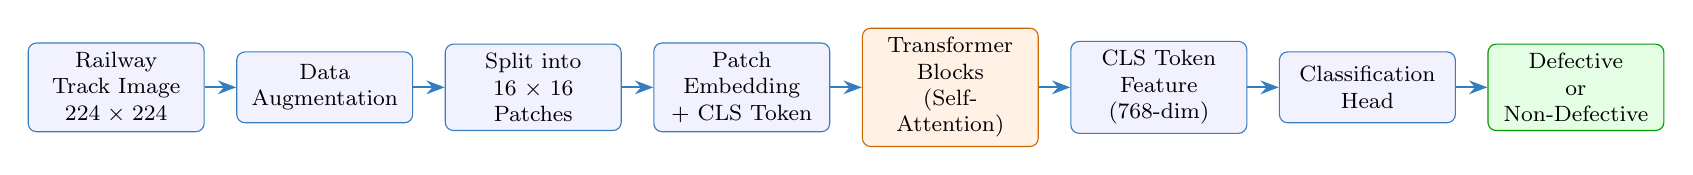
\begin{tikzpicture}[
    node distance=0.6cm and 0.4cm,
    block/.style={rectangle, draw=cvprblue, fill=blue!5, text width=2.0cm, minimum height=0.9cm, align=center, rounded corners=3pt, font=\footnotesize},
    phase/.style={rectangle, draw=orange!80!black, fill=orange!10, text width=2.0cm, minimum height=0.9cm, align=center, rounded corners=3pt, font=\footnotesize},
    output/.style={rectangle, draw=green!60!black, fill=green!10, text width=2.0cm, minimum height=0.9cm, align=center, rounded corners=3pt, font=\footnotesize},
    arrow/.style={-Stealth, thick, cvprblue},
]
    \node[block] (input) {Railway\\Track Image\\$224\times224$};
    \node[block, right=of input] (aug) {Data\\Augmentation};
    \node[block, right=of aug] (patch) {Split into\\$16\times16$\\Patches};
    \node[block, right=of patch] (embed) {Patch\\Embedding\\+ CLS Token};
    \node[phase, right=of embed] (blocks) {Transformer\\Blocks\\(Self-Attention)};
    \node[block, right=of blocks] (cls) {CLS Token\\Feature\\(768-dim)};
    \node[block, right=of cls] (head) {Classification\\Head};
    \node[output, right=of head] (out) {Defective\\or\\Non-Defective};
    
    \draw[arrow] (input) -- (aug);
    \draw[arrow] (aug) -- (patch);
    \draw[arrow] (patch) -- (embed);
    \draw[arrow] (embed) -- (blocks);
    \draw[arrow] (blocks) -- (cls);
    \draw[arrow] (cls) -- (head);
    \draw[arrow] (head) -- (out);
\end{tikzpicture}
\caption{\textbf{Pipeline overview.} A railway track image is augmented, split into 196 patches of size $16\times16$, passed through transformer blocks with self-attention, and classified as defective or non-defective using the CLS token output.}
\label{fig:overview}
\end{figure*}

\subsection{How Vision Transformers Work}

Unlike CNNs which use convolutional filters, a ViT works by:
\begin{enumerate}[leftmargin=*, itemsep=2pt]
    \item \textbf{Splitting the image into patches:} A $224\times224$ image is divided into $14 \times 14 = 196$ non-overlapping patches of $16 \times 16$ pixels each.
    \item \textbf{Embedding patches:} Each patch is flattened and projected into an embedding vector. A special \texttt{[CLS]} (classification) token is added. Positional embeddings tell the model where each patch is located.
    \item \textbf{Self-Attention:} In each transformer block, every patch looks at every other patch through self-attention. This allows the model to relate distant parts of the image---for example, connecting a crack in one corner to the overall track structure.
    \item \textbf{Classification:} The \texttt{[CLS]} token at the output captures a summary of the entire image and is fed into a classification head to produce the final prediction.
\end{enumerate}


\subsection{Approach A: ViT From Scratch (Akash Tiwari)}

In this approach, we build a lightweight ViT entirely from scratch using PyTorch---no pretrained weights are used. The idea is to see how well a small transformer can learn from only 300 images when trained from random initialization.

\paragraph{Architecture.}
The model has 6 transformer blocks, 4 attention heads, and uses 128-dimensional embeddings. With only \textbf{919,170 parameters}, it is much smaller than standard ViTs (ViT-B/16 has 86 million parameters). This makes it less prone to overfitting on small datasets but also limits its ability to learn complex features.

\paragraph{Training.}
The model is trained for 30 epochs using:
\begin{itemize}[leftmargin=*, itemsep=1pt]
    \item AdamW optimizer with learning rate $3 \times 10^{-4}$ and weight decay $10^{-2}$
    \item CrossEntropyLoss (since this uses 2-class output)
    \item Cosine annealing learning rate schedule
    \item Basic augmentation: horizontal flip, rotation ($\pm15\degree$), color jitter, random translation
\end{itemize}


\subsection{Approach B: Pretrained ViT-B/16 with Fine-Tuning (Vaibhav Soni)}

In this approach, we start with a ViT-B/16 that has already been trained on ImageNet-21k (14 million images). Since this model has already learned to understand images in general, we only need to teach it to recognize railway track defects specifically.

\paragraph{Architecture.}
We use the full ViT-B/16 from the \texttt{timm} library~\cite{Wightman2021}: 12 transformer blocks, 12 attention heads, 768-dimensional embeddings, totaling \textbf{86 million parameters}. We replace the default classification head with a custom head:
$$\text{LayerNorm} \to \text{Dense}(256) \to \text{GELU} \to \text{Dropout} \to \text{Dense}(1) \to \text{Sigmoid}$$

\paragraph{Two-Phase Training Strategy.}
Since the model is so large compared to our dataset, we train it carefully in two phases:

\textbf{Phase 1 --- Train the head only (15 epochs):}
We freeze the entire pretrained backbone (no weight updates) and only train the classification head. This prevents the large model from immediately overfitting.
\begin{itemize}[leftmargin=*, itemsep=1pt]
    \item Learning rate: $10^{-3}$
    \item Scheduler: Cosine annealing ($\eta_{min} = 10^{-6}$)
\end{itemize}

\textbf{Phase 2 --- Fine-tune the top half (up to 30 epochs):}
Starting from the best Phase~1 model, we unfreeze the top 6 of 12 transformer blocks. The key idea is to use \textit{different learning rates}: a very small learning rate ($5 \times 10^{-6}$) for the backbone to avoid destroying pretrained features, and a larger rate ($10^{-4}$) for the head.
\begin{itemize}[leftmargin=*, itemsep=1pt]
    \item Early stopping with patience of 10 epochs
    \item Gradient clipping at 1.0 to prevent training instability
    \item Cosine annealing with warm restarts
\end{itemize}


\subsection{Architecture Comparison}

Table~\ref{tab:arch} summarizes the key differences between the two approaches.

\begin{table}[h]
\centering
\caption{Comparison of the two ViT architectures.}
\label{tab:arch}
\small
\begin{tabular}{lcc}
\toprule
\textbf{Property} & \textbf{Approach A} & \textbf{Approach B} \\
& \textbf{(From Scratch)} & \textbf{(Pretrained)} \\
\midrule
Embed.\ Dimension & 128 & 768 \\
Attention Heads & 4 & 12 \\
Transformer Blocks & 6 & 12 \\
MLP Hidden Dim & 256 & 3072 \\
Total Parameters & 919K & 86M \\
Pretrained? & No & Yes (ImageNet-21k) \\
Output Format & 2-class softmax & Binary sigmoid \\
Training Strategy & Single phase & Two-phase \\
\bottomrule
\end{tabular}
\end{table}


\subsection{Data Augmentation}

Both approaches use data augmentation to increase the effective size of the training set. Approach~B uses a more aggressive augmentation pipeline (Table~\ref{tab:aug}), designed specifically for railway inspection conditions.

\begin{table}[h]
\centering
\caption{Augmentation comparison. Approach B uses more augmentations tailored to railway conditions.}
\label{tab:aug}
\small
\begin{tabular}{lcc}
\toprule
\textbf{Augmentation} & \textbf{A} & \textbf{B} \\
\midrule
Horizontal flip & \checkmark & \checkmark \\
Random rotation & \checkmark & \checkmark \\
Color jitter & \checkmark & \checkmark \\
Random translation & \checkmark & \checkmark \\
Vertical flip & & \checkmark \\
Perspective distortion & & \checkmark \\
Gaussian noise & & \checkmark \\
Gaussian blur & & \checkmark \\
Motion blur & & \checkmark \\
CLAHE (crack enhancement) & & \checkmark \\
Coarse dropout (occlusion) & & \checkmark \\
\bottomrule
\end{tabular}
\end{table}

CLAHE (Contrast Limited Adaptive Histogram Equalization) is particularly useful because it enhances the visibility of fine cracks that might be hard to see under uneven lighting. Motion blur simulates images taken from a moving inspection vehicle.


\subsection{Test-Time Augmentation (TTA)}

In Approach~B, during testing we don't just predict once per image. Instead, we create 7 augmented versions of each test image, run predictions on all of them, and average the results:
$$\hat{p}_{TTA} = \frac{1}{8}\left(p_{original} + \sum_{i=1}^{7} p_{augmented,i}\right)$$
This reduces the effect of random variations and gives more stable predictions.


\subsection{Explainability: Grad-CAM and Attention Maps}

For a safety application like railway inspection, it's important to understand \textit{why} the model makes a prediction. We use:
\begin{itemize}[leftmargin=*, itemsep=2pt]
    \item \textbf{Grad-CAM}~\cite{Selvaraju2017}: Generates heatmaps showing which parts of the image contribute most to the prediction. We adapt this for ViT by reshaping patch tokens into a spatial grid.
    \item \textbf{Self-Attention Maps}: Visualize which patches the CLS token attends to, revealing whether the model is looking at defect regions or irrelevant background.
\end{itemize}


%=========================================================
% 5. EXPERIMENTS AND RESULTS
%=========================================================
\section{Experiments and Results}

\subsection{Setup}

Both approaches use:
\begin{itemize}[leftmargin=*, itemsep=1pt]
    \item Image size: $224 \times 224$ pixels
    \item Batch size: 16
    \item ImageNet normalization ($\mu = [0.485, 0.456, 0.406]$, $\sigma = [0.229, 0.224, 0.225]$)
    \item Reproducibility seed: 42
\end{itemize}

Approach~B additionally uses mixed precision training (FP16) for faster computation and gradient clipping for training stability.


\subsection{Approach A Results: From-Scratch ViT}

The from-scratch ViT was trained for 30 epochs with cosine annealing.

\begin{itemize}[leftmargin=*, itemsep=2pt]
    \item \textbf{Best Validation Accuracy:} 80.65\% (at Epoch 16)
    \item \textbf{Final Training Accuracy:} $\sim$82\% (at Epoch 30)
\end{itemize}

% ── PLACEHOLDER: Approach A Training Curves ──
\begin{figure}[h]
\centering
\fbox{\parbox{0.93\linewidth}{\centering\vspace{1.5cm}
\textit{[To be added: Training loss and accuracy\\curves for Approach A (from-scratch ViT)]}
\vspace{1.5cm}}}
\caption{Training and validation curves for Approach A (from-scratch ViT, 30 epochs).}
\label{fig:approach_a_curves}
\end{figure}


\subsection{Approach B Results: Pretrained ViT-B/16}

\paragraph{Phase 1 (Frozen Backbone, 15 epochs):}
The classification head converged quickly, reaching 80.65\% validation accuracy. Training accuracy saturated at $\sim$82\%, showing that the pretrained features are already quite useful even without fine-tuning.

\paragraph{Phase 2 (Fine-tuning, 12/30 epochs):}
After unfreezing the top 6 transformer blocks, training continued for 12 epochs before early stopping. Table~\ref{tab:phase2} shows the key epochs.

\begin{table}[h]
\centering
\caption{Approach B, Phase 2 training progress. Best model at Epoch 2 (val loss = 0.402). Early stopping triggered at Epoch 12.}
\label{tab:phase2}
\small
\begin{tabular}{ccccc}
\toprule
\textbf{Ep.} & \textbf{Train Loss} & \textbf{Train Acc} & \textbf{Val Loss} & \textbf{Val Acc} \\
\midrule
1 & 0.362 & 81.9\% & 0.511 & 80.7\% \\
2 & 0.299 & 86.0\% & \textbf{0.402} & 80.7\% \\
5 & 0.270 & 89.0\% & 0.424 & 79.0\% \\
8 & 0.198 & 92.3\% & 0.408 & 80.7\% \\
12 & 0.219 & 89.6\% & 0.443 & 79.0\% \\
\bottomrule
\end{tabular}
\end{table}

A notable observation is that by Epoch~8, training accuracy reached 92.3\% while validation stayed at 80.7\%---a gap of about 12\%. This indicates overfitting, which is expected given only 300 training images for an 86M-parameter model.

% ── PLACEHOLDER: Approach B Training Curves ──
\begin{figure}[h]
\centering
\fbox{\parbox{0.93\linewidth}{\centering\vspace{1.5cm}
\textit{[To be added: Training history plots for Approach B\\(loss, accuracy, recall, F1, learning rate, overfitting gap)]}
\vspace{1.5cm}}}
\caption{Training history for Approach B showing Phase 1 and Phase 2 with phase boundary indicated.}
\label{fig:approach_b_curves}
\end{figure}


\subsection{Test Set Comparison}

Table~\ref{tab:results} compares both approaches on the held-out test set (22 images).

\begin{table}[h]
\centering
\caption{Test set results. Approach B with TTA achieves the best F1 score.}
\label{tab:results}
\small
\begin{tabular}{lccccc}
\toprule
\textbf{Method} & \textbf{Acc} & \textbf{Prec} & \textbf{Rec} & \textbf{F1} & \textbf{AUC} \\
\midrule
\textbf{A:} From-Scratch & 77.3\% & 0.73 & 0.73 & 0.73 & --- \\
\textbf{B:} Pretrained & 72.7\% & 0.86 & 0.55 & 0.67 & 0.826 \\
\textbf{B:} Pretrained + TTA & \textbf{80.7\%} & \textbf{0.86} & \textbf{0.87} & \textbf{0.83} & \textbf{0.826} \\
\bottomrule
\end{tabular}
\end{table}

\paragraph{Key observations:}

\begin{enumerate}[leftmargin=*, itemsep=3pt]
    \item \textbf{Approach A gives balanced results:} The from-scratch ViT achieves 77.3\% accuracy with roughly equal precision and recall (both $\sim$0.73). This means it makes mistakes in both directions equally---sometimes misses defects, sometimes raises false alarms.
    
    \item \textbf{Approach B without TTA is conservative:} The pretrained ViT has high precision (0.86) but low recall (0.55). It correctly identifies defects when it flags them, but \textit{misses about 45\% of actual defects}. For railway safety, this is problematic because a missed crack is far more dangerous than a false alarm.
    
    \item \textbf{TTA dramatically improves recall:} Adding Test-Time Augmentation boosts recall from 0.55 to 0.87---a 58\% improvement. By averaging predictions across 8 versions of each image, the model becomes much less likely to miss actual defects.
    
    \item \textbf{AUC-ROC of 0.826:} This shows the model can rank images well---it understands the difference between defective and non-defective, even if the 0.5 threshold isn't optimal.
    
    \item \textbf{Small test set caveat:} With only 22 test images, each misclassification changes accuracy by 4.5\%. The metrics should be interpreted with this in mind.
\end{enumerate}

% ── PLACEHOLDER: Evaluation Plots ──
\begin{figure}[h]
\centering
\fbox{\parbox{0.93\linewidth}{\centering\vspace{1.5cm}
\textit{[To be added: Evaluation plots ---\\confusion matrix, ROC curve, PR curve,\\confidence distribution, metrics bar chart]}
\vspace{1.5cm}}}
\caption{Test set evaluation visualizations for Approach B (pretrained ViT-B/16 with TTA).}
\label{fig:evaluation}
\end{figure}


\subsection{Discussion: Which Approach Is Better?}

Neither approach is strictly better than the other---they offer different trade-offs:

\begin{table}[h]
\centering
\caption{Trade-off comparison between the two approaches.}
\label{tab:tradeoff}
\small
\begin{tabular}{lcc}
\toprule
\textbf{Factor} & \textbf{A (From Scratch)} & \textbf{B (Pretrained)} \\
\midrule
Best test F1 & 0.73 & \textbf{0.83 (with TTA)} \\
Parameters & \textbf{919K} & 86M \\
Needs pretrained weights? & \textbf{No} & Yes \\
Training time & \textbf{Fast} & Slow \\
Inference speed & \textbf{Fast} & 8x slower (with TTA) \\
Overfitting risk & \textbf{Low} & High \\
Best for & Learning/edge devices & Maximum accuracy \\
\bottomrule
\end{tabular}
\end{table}

The pretrained ViT with TTA gives the best raw performance (F1 = 0.83), but the from-scratch ViT (F1 = 0.73) is impressive considering it was trained from random initialization on just 300 images. This demonstrates that even a lightweight transformer \textit{can} learn useful visual patterns from very little data.


\subsection{Explainability Results}

% ── PLACEHOLDER: Grad-CAM Results ──
\begin{figure}[h]
\centering
\fbox{\parbox{0.93\linewidth}{\centering\vspace{1.5cm}
\textit{[To be added: Grad-CAM heatmaps\\showing where the model looks on\\defective vs.\ non-defective track images]}
\vspace{1.5cm}}}
\caption{Grad-CAM heatmaps. For defective tracks, the model focuses on crack regions. For non-defective tracks, attention is spread more evenly across the surface.}
\label{fig:gradcam}
\end{figure}

% ── PLACEHOLDER: Attention Maps ──
\begin{figure}[h]
\centering
\fbox{\parbox{0.93\linewidth}{\centering\vspace{1.5cm}
\textit{[To be added: Self-attention maps\\from the last transformer block, showing\\CLS token attention across patches]}
\vspace{1.5cm}}}
\caption{Self-attention maps from the last transformer block. Different heads specialize in different aspects: some focus on the rail structure, others on the surrounding area.}
\label{fig:attention}
\end{figure}

The Grad-CAM and attention visualizations confirm that:
\begin{itemize}[leftmargin=*, itemsep=2pt]
    \item For correctly classified \textbf{defective} tracks, the model focuses on crack regions, surface breaks, and structural damage.
    \item For \textbf{non-defective} tracks, attention is distributed more evenly across the rail surface.
    \item Misclassifications tend to occur on images with subtle cracks (missed defects) or heavy rust/discoloration (false alarms).
\end{itemize}

% ── PLACEHOLDER: Misclassification Analysis ──
\begin{figure}[h]
\centering
\fbox{\parbox{0.93\linewidth}{\centering\vspace{1.5cm}
\textit{[To be added: Misclassified images\\with Grad-CAM overlays showing\\why the model got confused]}
\vspace{1.5cm}}}
\caption{Misclassification analysis with Grad-CAM. The model struggles with subtle cracks and heavy rust that mimics defect appearance.}
\label{fig:misclass}
\end{figure}


%=========================================================
% 6. CONCLUSION
%=========================================================
\section{Conclusion}

In this project, we applied Vision Transformers to the task of railway track fault detection. We compared two approaches:

\begin{itemize}[leftmargin=*, itemsep=2pt]
    \item \textbf{Approach A (From Scratch):} A lightweight ViT with 919K parameters achieves 77.3\% accuracy and balanced precision/recall, showing that transformers can learn from very small datasets.
    \item \textbf{Approach B (Pretrained + Fine-tuned):} A ViT-B/16 pretrained on ImageNet-21k, fine-tuned with a two-phase strategy and evaluated with TTA, achieves the best performance at 80.7\% accuracy and 0.83 F1 score.
\end{itemize}

The biggest challenge throughout was the \textbf{extremely small dataset} (384 total images). Our results show that with the right training strategies (progressive fine-tuning, aggressive augmentation, TTA), ViTs can be effective even in data-scarce scenarios.

\paragraph{Future Work.}
\begin{enumerate}[leftmargin=*, itemsep=2pt]
    \item Collecting a larger dataset with more diverse defect types and severity levels
    \item Trying hybrid architectures like Swin Transformer~\cite{Liu2021} that combine local and global attention
    \item Optimizing for real-time inference on edge devices for deployment in inspection vehicles
    \item Tuning the classification threshold based on the ROC curve to maximize recall for safety-critical applications
\end{enumerate}

%=========================================================
% REFERENCES
%=========================================================
{\small
\bibliographystyle{ieee_fullname}
\begin{thebibliography}{15}

\bibitem{Dosovitskiy2021}
A.~Dosovitskiy, L.~Beyer, A.~Kolesnikov, D.~Weissenborn, X.~Zhai, T.~Unterthiner, M.~Dehghani, M.~Minderer, G.~Heigold, S.~Gelly, J.~Uszkoreit, and N.~Houlsby.
\newblock An image is worth 16x16 words: Transformers for image recognition at scale.
\newblock In \textit{Proc.\ ICLR}, 2021.

\bibitem{He2016}
K.~He, X.~Zhang, S.~Ren, and J.~Sun.
\newblock Deep residual learning for image recognition.
\newblock In \textit{Proc.\ CVPR}, pages 770--778, 2016.

\bibitem{Tan2019}
M.~Tan and Q.~V.~Le.
\newblock EfficientNet: Rethinking model scaling for convolutional neural networks.
\newblock In \textit{Proc.\ ICML}, 2019.

\bibitem{Touvron2021}
H.~Touvron, M.~Cord, M.~Douze, F.~Massa, A.~Sablayrolles, and H.~J{\'e}gou.
\newblock Training data-efficient image transformers \& distillation through attention.
\newblock In \textit{Proc.\ ICML}, 2021.

\bibitem{Selvaraju2017}
R.~R.~Selvaraju, M.~Cogswell, A.~Das, R.~Vedantam, D.~Parikh, and D.~Batra.
\newblock Grad-CAM: Visual explanations from deep networks via gradient-based localization.
\newblock In \textit{Proc.\ ICCV}, pages 618--626, 2017.

\bibitem{Buslaev2020}
A.~Buslaev, V.~I.~Iglovikov, E.~Khvedchenya, A.~Parinov, M.~Druzhinin, and A.~A.~Kalinin.
\newblock Albumentations: Fast and flexible image augmentations.
\newblock \textit{Information}, 11(2):125, 2020.

\bibitem{Deng2009}
J.~Deng, W.~Dong, R.~Socher, L.-J.~Li, K.~Li, and L.~Fei-Fei.
\newblock ImageNet: A large-scale hierarchical image database.
\newblock In \textit{Proc.\ CVPR}, pages 248--255, 2009.

\bibitem{Wightman2021}
R.~Wightman.
\newblock PyTorch Image Models.
\newblock \url{https://github.com/huggingface/pytorch-image-models}, 2021.

\bibitem{Dalal2005}
N.~Dalal and B.~Triggs.
\newblock Histograms of oriented gradients for human detection.
\newblock In \textit{Proc.\ CVPR}, pages 886--893, 2005.

\bibitem{Liu2021}
Z.~Liu, Y.~Lin, Y.~Cao, H.~Hu, Y.~Wei, Z.~Zhang, S.~Lin, and B.~Guo.
\newblock Swin Transformer: Hierarchical vision transformer using shifted windows.
\newblock In \textit{Proc.\ ICCV}, pages 10012--10022, 2021.

\bibitem{RailwayDataset}
Railway Track Fault Detection Dataset.
\newblock Available on Kaggle.
\newblock \url{https://www.kaggle.com/datasets/}.

\end{thebibliography}
}

%=========================================================
% APPENDIX
%=========================================================
\clearpage
\onecolumn
\appendix

\section{GitHub Repository}
\begin{center}
\url{https://github.com/akashcoder-collab/railway-track-fault-detection-vit}
\end{center}

\section{Datasets and Libraries Used}
\textbf{Datasets:}
\begin{itemize}
    \item Railway Track Fault Detection Dataset: \url{https://www.kaggle.com/datasets/}
    \item ImageNet-21k (used via pretrained weights): \url{https://www.image-net.org/}
\end{itemize}

\textbf{Libraries:}
\begin{itemize}
    \item PyTorch: \url{https://pytorch.org/}
    \item timm (PyTorch Image Models): \url{https://github.com/huggingface/pytorch-image-models}
    \item Albumentations: \url{https://github.com/albumentations-team/albumentations}
    \item pytorch-grad-cam: \url{https://github.com/jacobgil/pytorch-grad-cam}
    \item scikit-learn: \url{https://scikit-learn.org/}
\end{itemize}


\section{Code: Approach A --- ViT From Scratch (Akash Tiwari)}

\begin{lstlisting}[caption={From-scratch ViT implementation.}]
import torch
import torch.nn as nn
from torchvision.datasets import ImageFolder
from torch.utils.data import DataLoader
import torchvision.transforms as transforms
from sklearn.metrics import classification_report, confusion_matrix
import numpy as np

device = torch.device("cuda" if torch.cuda.is_available() else "cpu")

# Hyperparameters
num_classes = 2
batch_size = 16
img_size = 224
patch_size = 16
embedding_dim = 128
attention_heads = 4
transformer_blocks = 6
mlp_hidden_nodes = 256
learning_rate = 3e-4
epochs = 30
dropout_rate = 0.1
num_patches = (img_size // patch_size) ** 2  # 196

# Augmentation
train_transform = transforms.Compose([
    transforms.Resize((img_size, img_size)),
    transforms.RandomHorizontalFlip(),
    transforms.RandomRotation(15),
    transforms.ColorJitter(brightness=0.2, contrast=0.2, saturation=0.2),
    transforms.RandomAffine(degrees=0, translate=(0.1, 0.1)),
    transforms.ToTensor(),
    transforms.Normalize(mean=[0.485, 0.456, 0.406], std=[0.229, 0.224, 0.225]),
])

class PatchEmbeddings(nn.Module):
    def __init__(self):
        super().__init__()
        self.patch_embed = nn.Conv2d(3, embedding_dim,
                                     kernel_size=patch_size, stride=patch_size)
    def forward(self, x):
        return self.patch_embed(x).flatten(2).transpose(1, 2)

class TransformerEncoder(nn.Module):
    def __init__(self):
        super().__init__()
        self.norm1 = nn.LayerNorm(embedding_dim)
        self.norm2 = nn.LayerNorm(embedding_dim)
        self.attn = nn.MultiheadAttention(embedding_dim, attention_heads,
                                          dropout=dropout_rate, batch_first=True)
        self.mlp = nn.Sequential(
            nn.Linear(embedding_dim, mlp_hidden_nodes), nn.GELU(),
            nn.Dropout(dropout_rate),
            nn.Linear(mlp_hidden_nodes, embedding_dim), nn.Dropout(dropout_rate))

    def forward(self, x):
        res = x; x = self.norm1(x); x, _ = self.attn(x, x, x); x = x + res
        res = x; x = self.norm2(x); x = self.mlp(x); x = x + res
        return x

class VisionTransformer(nn.Module):
    def __init__(self):
        super().__init__()
        self.patch_embedding = PatchEmbeddings()
        self.cls_token = nn.Parameter(torch.randn(1, 1, embedding_dim))
        self.pos_embedding = nn.Parameter(torch.randn(1, num_patches + 1, embedding_dim))
        self.pos_drop = nn.Dropout(dropout_rate)
        self.transformer = nn.Sequential(
            *[TransformerEncoder() for _ in range(transformer_blocks)])
        self.mlp_head = nn.Sequential(
            nn.LayerNorm(embedding_dim), nn.Linear(embedding_dim, num_classes))

    def forward(self, x):
        x = self.patch_embedding(x)
        cls = self.cls_token.expand(x.size(0), -1, -1)
        x = self.pos_drop(torch.cat((cls, x), dim=1) + self.pos_embedding)
        x = self.transformer(x)
        return self.mlp_head(x[:, 0])  # CLS token output

# Training
model = VisionTransformer().to(device)
optimizer = torch.optim.AdamW(model.parameters(), lr=learning_rate, weight_decay=1e-2)
criterion = nn.CrossEntropyLoss()
scheduler = torch.optim.lr_scheduler.CosineAnnealingLR(optimizer, T_max=epochs)
\end{lstlisting}


\section{Code: Approach B --- Pretrained ViT-B/16 (Vaibhav Soni)}

\begin{lstlisting}[caption={Pretrained ViT-B/16 with two-phase fine-tuning (key components).}]
import timm
import albumentations as A
from albumentations.pytorch import ToTensorV2
from torch.amp import autocast, GradScaler

class RailwayViT(nn.Module):
    def __init__(self, model_name='vit_base_patch16_224', pretrained=True):
        super().__init__()
        self.backbone = timm.create_model(model_name, pretrained=pretrained,
                                           num_classes=0, drop_rate=0.1)
        feat_dim = self.backbone.num_features  # 768
        self.head = nn.Sequential(
            nn.LayerNorm(feat_dim),
            nn.Linear(feat_dim, 256), nn.GELU(), nn.Dropout(0.3),
            nn.Linear(256, 128), nn.GELU(), nn.Dropout(0.21),
            nn.Linear(128, 1))

    def freeze_backbone(self):
        for p in self.backbone.parameters(): p.requires_grad = False

    def unfreeze_backbone(self, ratio=0.5):
        for p in self.backbone.parameters(): p.requires_grad = True
        for p in self.backbone.patch_embed.parameters(): p.requires_grad = False
        blocks = list(self.backbone.blocks)
        for b in blocks[:int(len(blocks) * (1 - ratio))]:
            for p in b.parameters(): p.requires_grad = False

    def forward(self, x):
        return self.head(self.backbone(x))

# --- Phase 1: Frozen backbone ---
model.freeze_backbone()
opt1 = optim.AdamW(filter(lambda p: p.requires_grad, model.parameters()),
                   lr=1e-3, weight_decay=1e-4)
sched1 = optim.lr_scheduler.CosineAnnealingLR(opt1, T_max=15, eta_min=1e-6)
# Train 15 epochs...

# --- Phase 2: Unfreeze top 50% with layer-wise LR ---
model.unfreeze_backbone(ratio=0.5)
opt2 = optim.AdamW([
    {'params': backbone_params, 'lr': 5e-6},   # Small LR for backbone
    {'params': model.head.parameters(), 'lr': 1e-4}  # Larger LR for head
], weight_decay=1e-4)
# Train up to 30 epochs with early stopping...

# --- Test-Time Augmentation ---
def evaluate_with_tta(model, dataset, n_augments=7):
    for idx in range(len(dataset)):
        probs = [predict(original)]
        for _ in range(n_augments):
            probs.append(predict(augment(original)))
        final_prob = np.mean(probs)
\end{lstlisting}


\end{document}
